% Created with jtex v.1.0.12
\documentclass[twocolumn, switch]{article}
\usepackage{preprint}
\usepackage{hyperref}
\usepackage[numbers,square]{natbib}

%%%%%%%%%%%%%%%%%%%%%%%%%%%%%%%%%%%%%%%%%%%%%%%%%%
%%%%%%%%%%%%%%%%%%%%  imports  %%%%%%%%%%%%%%%%%%%
\usepackage{amsmath}
\usepackage{booktabs}
\usepackage{graphicx}
%%%%%%%%%%%%%%%%%%%%%%%%%%%%%%%%%%%%%%%%%%%%%%%%%%
\usepackage{glossaries}
\makeglossaries

%%%%%%%%%%%%%%%%%%%%%%%%%%%%%%%%%%%%%%%%%%%%%%%%%%
%%%%%%%%%%%%%%%%%%%  acronyms  %%%%%%%%%%%%%%%%%%%
\newacronym{ussr}{USSR}{Soviet Union}
%%%%%%%%%%%%%%%%%%%%%%%%%%%%%%%%%%%%%%%%%%%%%%%%%%



% colors for hyperlinks
\hypersetup{colorlinks=true, linkcolor=purple, urlcolor=blue, citecolor=cyan, anchorcolor=black}

\usepackage[utf8]{inputenc}	% allow utf-8 input
\usepackage[T1]{fontenc}
\usepackage{xcolor}
\usepackage{lineno}					% Line numbers
\usepackage{tikz} 					% ORCiD insertion

%% Bibliography options
\bibliographystyle{unsrtnat}

 %% Special figure caption options
\usepackage{newfloat}
\DeclareFloatingEnvironment[name={Supplementary Figure}]{suppfigure}
\usepackage{sidecap}
\sidecaptionvpos{figure}{c}

% Section title spacing  options
\usepackage{titlesec}
\titlespacing\section{0pt}{12pt plus 3pt minus 3pt}{1pt plus 1pt minus 1pt}
\titlespacing\subsection{0pt}{10pt plus 3pt minus 3pt}{1pt plus 1pt minus 1pt}
\titlespacing\subsubsection{0pt}{8pt plus 3pt minus 3pt}{1pt plus 1pt minus 1pt}

\definecolor{lime}{HTML}{A6CE39}
\DeclareRobustCommand{\orcidicon}{
	
\begin{tikzpicture}
	\draw[lime, fill=lime] (0,0)
	circle [radius=0.16]
	node[white] {{\fontfamily{qag}\selectfont \tiny ID}};
	\draw[white, fill=white] (-0.0625,0.095)
	circle [radius=0.007];
	\end{tikzpicture}
	\hspace{-2mm}
}

%%%%%%%%%%%%%%%%   Title   %%%%%%%%%%%%%%%%
\title{Analysis on the Life Expectancies of Countries (1990-2021)}

% Add watermark with submission status
% Awaiting watermark support
% \usepackage{xwatermark}
% % Left watermark
% \newwatermark[firstpage,color=gray!60,angle=90,scale=0.32, xpos=-4.05in,ypos=0]{\href{https://doi.org/}{\color{gray}{Publication doi}}}
% % Right watermark
% \newwatermark[firstpage,color=gray!60,angle=90,scale=0.32, xpos=3.9in,ypos=0]{\href{https://doi.org/}{\color{gray}{Preprint doi}}}
% % Bottom watermark
% \newwatermark[firstpage,color=gray!90,angle=0,scale=0.28, xpos=0in,ypos=-5in]{*correspondence: \texttt{}}

%%%%%%%%%%%%%%%  Author list  %%%%%%%%%%%%%%%
\usepackage{authblk}
\renewcommand*{\Authfont}{\bfseries}

\author[1]{Neel Date & Pranav Nair}
\affil[1]{NCSSM}

%%%%%%%%%%%%%%    Front matter    %%%%%%%%%%%%%%
\begin{document}

\twocolumn[\begin{@twocolumnfalse}

\maketitle

\begin{abstract}
From 1990 to 2021, the world generally celebrated a consistent increase in average life expectancy. This increase was likely a result of numerous key factors, including: the expansion of medical infrastructure across the world (hospitals, vaccines, proper nutrition), the lack of major wars, and the overall increase in human happiness due to economic prosperity. However, not all countries attained an equitable increase in life expectancy, largely due to their pre-existing human development groups. A pandemic in 2020 was also responsible for the abrupt decline in life expectancy across the world, leading to speculation that the meteoric rise in life expectancy may not recover.\\
\end{abstract}

\keywords{}

\vspace{0.5cm}

\end{@twocolumnfalse}]

%%%%%%%%%%%%%%%  Main text   %%%%%%%%%%%%%%%

\subsection{Average Life Expectancy of the World (1990-2021)}

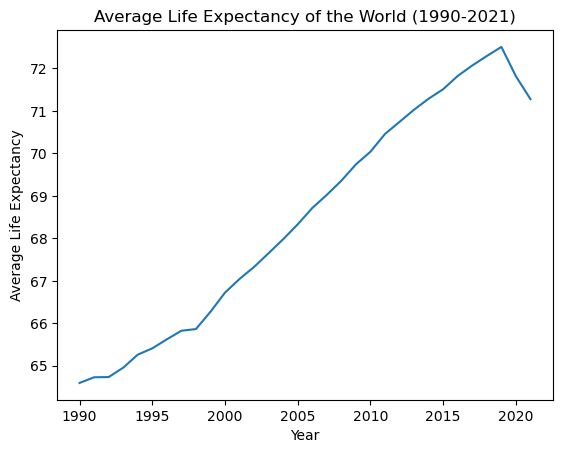
\includegraphics[width=0.7\linewidth]{files/8bb61c83fe12eb8d09a4741f1470b91f.png}

\paragraph{Consistent Growth}

As detailed in the line graph above, the average life expectancy of the world \textbf{consistently grew} from 1990-2019. Our team hypothesizes that the increase in life expectancy can be directly correlated with the economic and lifestyle advancements during this time period. The initial rise in the 1990s likely stemmed from more countries embracing free market capitalism after the collapse of the \acrshort{ussr}, increasing the purchasing power of millions of people. Furthermore, the effects of the Green Revolution were also present, with bountiful agricultural yields also increasing life expectancy by reducing the rate of famine.

\paragraph{A Year in Decline: The COVID-19 Pandemic}

The trend seen in the line graph came to an abrupt end in 2020, when the COVID-19 pandemic swept the world and killed millions of people. Although the actual causes of life expectancy decrease remained somewhat constant, the overall uptick in deaths across the world served to decrease average life expectancy considerably. Notably, the decrease affected all human development groups evenly, even countries that had access to better medical infrastructure.

\subsection{Comparing Life Expectancies Across Human Development Groups}

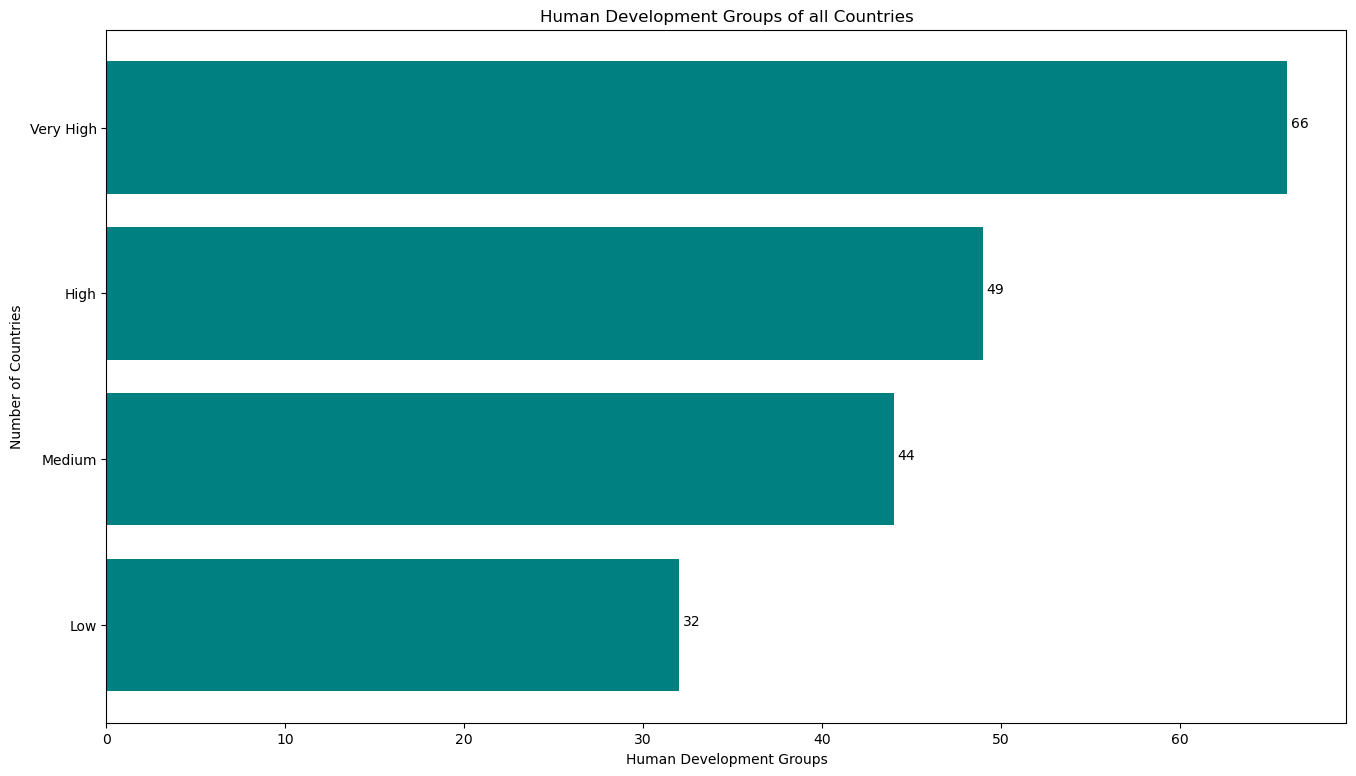
\includegraphics[width=0.7\linewidth]{files/490bc14e53c1c451efc0b8a57d512a7e.png}

\paragraph{Context}

As extrapolated from the bar graph above, countries can be divided into 4 Human Development Groups: Low, Medium, High, and Very High. The criteria for these Development Groups is based on a variety of factors, including quality of life, economic prosperity, and access to medical infrastructure. A majority of countries are placed into either the High or Very High groups, suggesting that they should also yield higher average life expectancies, whereas Low and Medium countries will generally have lower life expectancies. This conclusion is supported in the graph below:

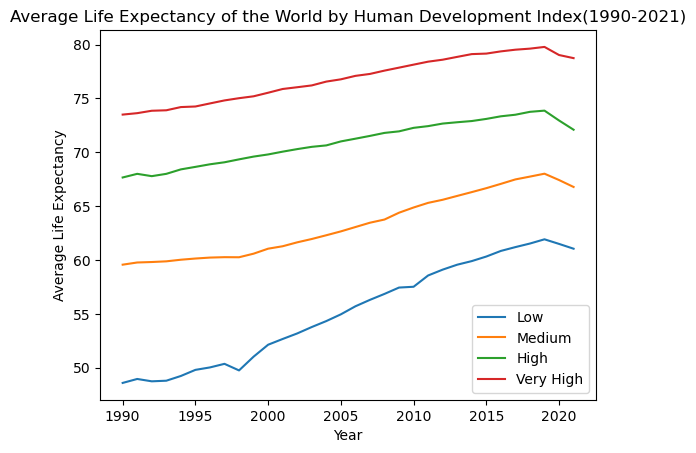
\includegraphics[width=0.7\linewidth]{files/ae930fdd7fbb8fa24ba29225b51cd6b8.png}

\subsection{Sample Data Set}

\begin{verbatim}
ISO3               Country Continent           Hemisphere  \
0  AFG           Afghanistan      Asia  Northern Hemisphere   
1  AGO                Angola    Africa  Southern Hemisphere   
2  ALB               Albania    Europe  Northern Hemisphere   
3  AND               Andorra    Europe  Northern Hemisphere   
4  ARE  United Arab Emirates      Asia  Northern Hemisphere   

  Human Development Groups UNDP Developing Regions  HDI Rank (2021)  \
0                      Low                      SA            180.0   
1                   Medium                     SSA            148.0   
2                     High                     ECA             67.0   
3                Very High                     NaN             40.0   
4                Very High                      AS             26.0   

   Life Expectancy at Birth (1990)  Life Expectancy at Birth (1991)  \
0                          45.9672                          46.6631   
1                          41.8933                          43.8127   
2                          73.1439                          73.3776   
3                          78.4063                          77.9805   
4                          71.9004                          72.2414   

   Life Expectancy at Birth (1992)  ...  Life Expectancy at Birth (2012)  \
0                          47.5955  ...                          61.9230   
1                          42.2088  ...                          58.6231   
2                          73.7148  ...                          78.0640   
3                          80.3241  ...                          82.9166   
4                          72.3062  ...                          78.7155   

   Life Expectancy at Birth (2013)  Life Expectancy at Birth (2014)  \
0                          62.4167                          62.5451   
1                          59.3074                          60.0397   
2                          78.1226                          78.4075   
3                          82.9343                          82.9483   
4                          78.8528                          79.0442   

   Life Expectancy at Birth (2015)  Life Expectancy at Birth (2016)  \
0                          62.6587                          63.1361   
1                          60.6546                          61.0923   
2                          78.6441                          78.8602   
3                          82.9534                          82.9671   
4                          79.2232                          79.3347   

   Life Expectancy at Birth (2017)  Life Expectancy at Birth (2018)  \
0                          63.0160                          63.0810   
1                          61.6798                          62.1438   
2                          79.0473                          79.1838   
3                          82.9803                          82.9923   
4                          79.5036                          79.6274   

   Life Expectancy at Birth (2019)  Life Expectancy at Birth (2020)  \
0                          63.5645                          62.5751   
1                          62.4484                          62.2612   
2                          79.2825                          76.9893   
3                          83.0039                          79.0234   
4                          79.7262                          78.9457   

   Life Expectancy at Birth (2021)  
0                          61.9824  
1                          61.6434  
2                          76.4626  
3                          80.3684  
4                          78.7104  

[5 rows x 39 columns]
\end{verbatim}

\subsection{Linear Regression}

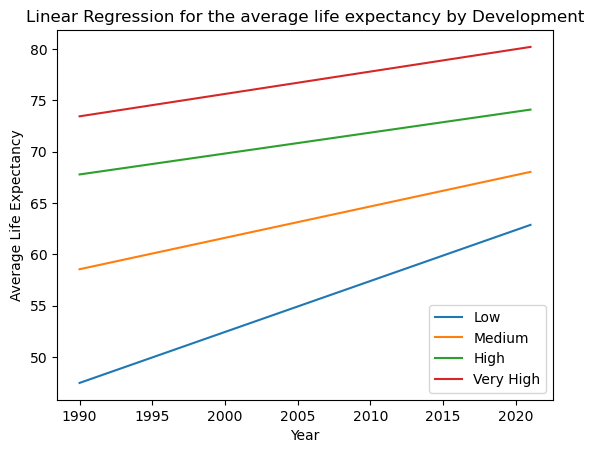
\includegraphics[width=0.7\linewidth]{files/2696926812c48737a0885ddaedea1dbc.png}

\begin{table}
\centering
\caption*{Average Growth In Life Expectancy by Human Development Level}
\begin{tabular}{p{\dimexpr 0.500\linewidth-2\tabcolsep}p{\dimexpr 0.500\linewidth-2\tabcolsep}}
\toprule
Human Development Level & Average Growth in Life Expectancy per annum \\
\hline
Low Development & 0.469 years \\
Medium Development & 0.306 years \\
High Development & 0.204 years \\
Very High Development & 0.218 years \\
\bottomrule
\end{tabular}
\end{table}

Using the graph, we can derive equations that project and model the growth of life expectancy per annum of a group of countries.

\begin{equation}
\label{my-equation}
\text{Low Development: } l = 0.469x + 47.487 \\
\text{Medium Development: } l = 0.306x + 58.552 \\
\text{High Development: } l = 0.204x + 67.775 \\
\text{Very High Development: } l = 0.218x + 73.432 \\


\\Where
\\
\\
\text{l = average life expectancy}\\
\text{x = years since 1990}\\
\end{equation}

Upon examining the overall linear regressions of each Human Development Group, two trends emerge: Firstly, despite an abrupt halt to life expectancy increase due to the COVID-19 Pandemic, all human development groups are still forecasted to grow their life expectancies into the future (perhaps at a decreased rate). Secondly, it is apparent that countries in the Low Human Development Group have undertaken a remarkable transformation in life expectancy increase, which is highlighted by the slope of the Low countries being the steepest. Our team suspects that this is due to the natural principle of diminishing returns: The higher a country starts out on the Human Development Index, the less potential it has for life expectancy growth, whereas countries designated as Low Development are destined to rapidly increase their life expectancies due to burgeoning technological and medical advancements.
%%%%%%%%%%%%%%%%%%%%%%%%%%%%%%%%%%%%%%%%%%%%%%%%%%
%%%%%%%%%%%%%%  acronyms & glossary  %%%%%%%%%%%%%
\printglossaries
%%%%%%%%%%%%%%%%%%%%%%%%%%%%%%%%%%%%%%%%%%%%%%%%%%




%%%%%%%%%%%%%%   Bibliography   %%%%%%%%%%%%%%

\end{document}
